\begin{center}
    \noindent \textbf{\large{Data Overview: Food Deliveries}} 
\end{center}

\noindent In this exam, we'll work with the DataFrame \texttt{orders}, which contains information about deliveries made using various food delivery services in India.

\vspace{.1in}

\noindent The first few rows of \texttt{orders} are shown below, but \texttt{orders} has many more rows than are shown.

% \vspace{-.5in}

\begin{center}

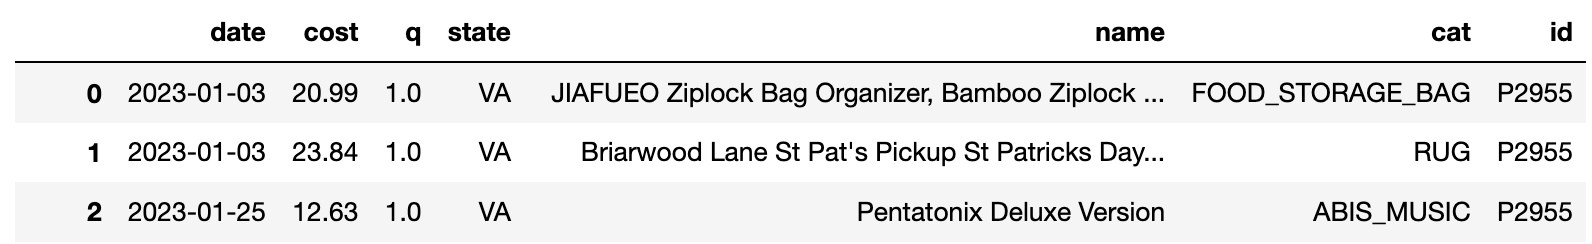
\includegraphics[width=0.7\textwidth]{midterm-images/df.png}

\end{center}

\vspace{.1in}

\noindent Each row in \texttt{orders} contains information about a single delivery. The columns in \texttt{orders} are as follows:

\begin{itemize}

\item \texttt{"driver" (str)}: The delivery driver's ID. Note that there are duplicate values in this column, because some drivers have made multiple deliveries.
\item \texttt{"type" (str)}: The type of food ordered; either \texttt{"Buffet"}, \texttt{"Drinks"}, \texttt{"Meal"}, or \texttt{"Snack"}.
\item \texttt{"rating" (float)}: The average rating of the driver out of 5, \textbf{after} making the given delivery.
\item \texttt{"dist" (float)}: The distance from the restaurant to the delivery address, in kilometers.
\item \texttt{"traffic" (str)}: The level of traffic; either \texttt{"High"}, \texttt{"Low"}, \texttt{"Moderate"}, or \texttt{"Very High"}.
\item \texttt{"minutes" (float)}: The time in minutes between when a customer places their order and when they receive it.

\end{itemize}

\noindent \textbf{Throughout the exam}, assume we have already run all necessary import statements.

\newpage

\noindent \textbf{Make sure you have read the Data Overview before beginning!}
